
\documentclass{beamer}

\usepackage{cmap}                                       % поиск в PDF
\usepackage[T2A]{fontenc}                       % кодировка
\usepackage[utf8]{inputenc}                     % кодировка исходного текста
\usepackage[english,russian]{babel}     % локализация и переносы

\usepackage{graphicx}
\graphicspath{{images/}}

%% \usetheme{Berkeley}
%% \usecolortheme{beaver}

\logo{
\includegraphics[height=0.8cm]{bsu_logo_ru.eps}}
\title{Элементы основ распознавания образов}
\author{Кузьмин А.А.}
\institute[]{\url{http://rfe.bsu.by/}}

\begin{document}

\begin{frame}
  \maketitle
\end{frame}

\section{Содержание}

\begin{frame} \label{cont}
  \frametitle{\insertsection}
  
  \begin{enumerate}
    \item Понять суть метода, позволяющего распознавать \pause
  \item Баланс между интуитивным пониманием и математическими формулировками \pause
  \item Тот случай, когда единственный способ заставить время лекции пролететь быстрее --- это стараться понимать то что рассказывает лектор \pause
  \item Требования для понимания курса \pause
    \begin{itemize}
      \item Теория вероятности
      \item Линейная алгебра
      \item Математический анализ
    \end{itemize}
  \end{enumerate}
\end{frame}

\section{Случайный вектор как модель сигнала}

%% Будем стараться быть проблема-ориентированными
\begin{frame}
  \frametitle{\insertsection}
  \framesubtitle{Описание сигнала при помощи вектора}
  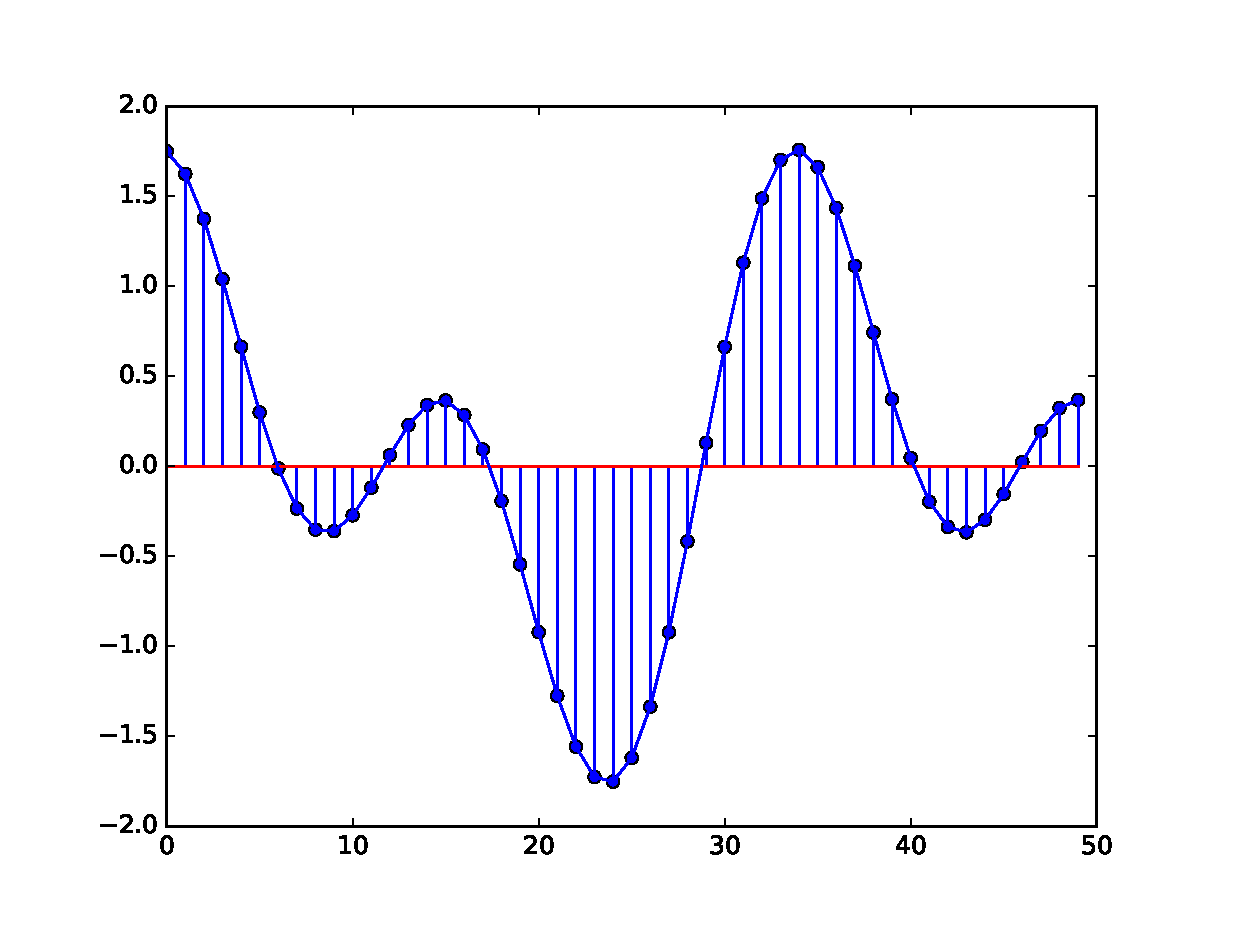
\includegraphics[width=0.8\textwidth]{tovec.eps}
\end{frame}

\begin{frame} \label{cont}
  \frametitle{\insertsection}
    \framesubtitle{Нотация}
  \begin{itemize}
    \item Последовательность: $x[n], n = 0, 1, \ldots, N - 1 $  \pause
    \item Вектор: $ \mathbf{x} = [x_0\,x_1 \ldots x_{N - 1}]^T $
  \end{itemize}
\end{frame}

\begin{frame}
  \frametitle{\insertsection}
  \framesubtitle{Выборка сигнала соответствующего звуку ``a'' номер 1}
  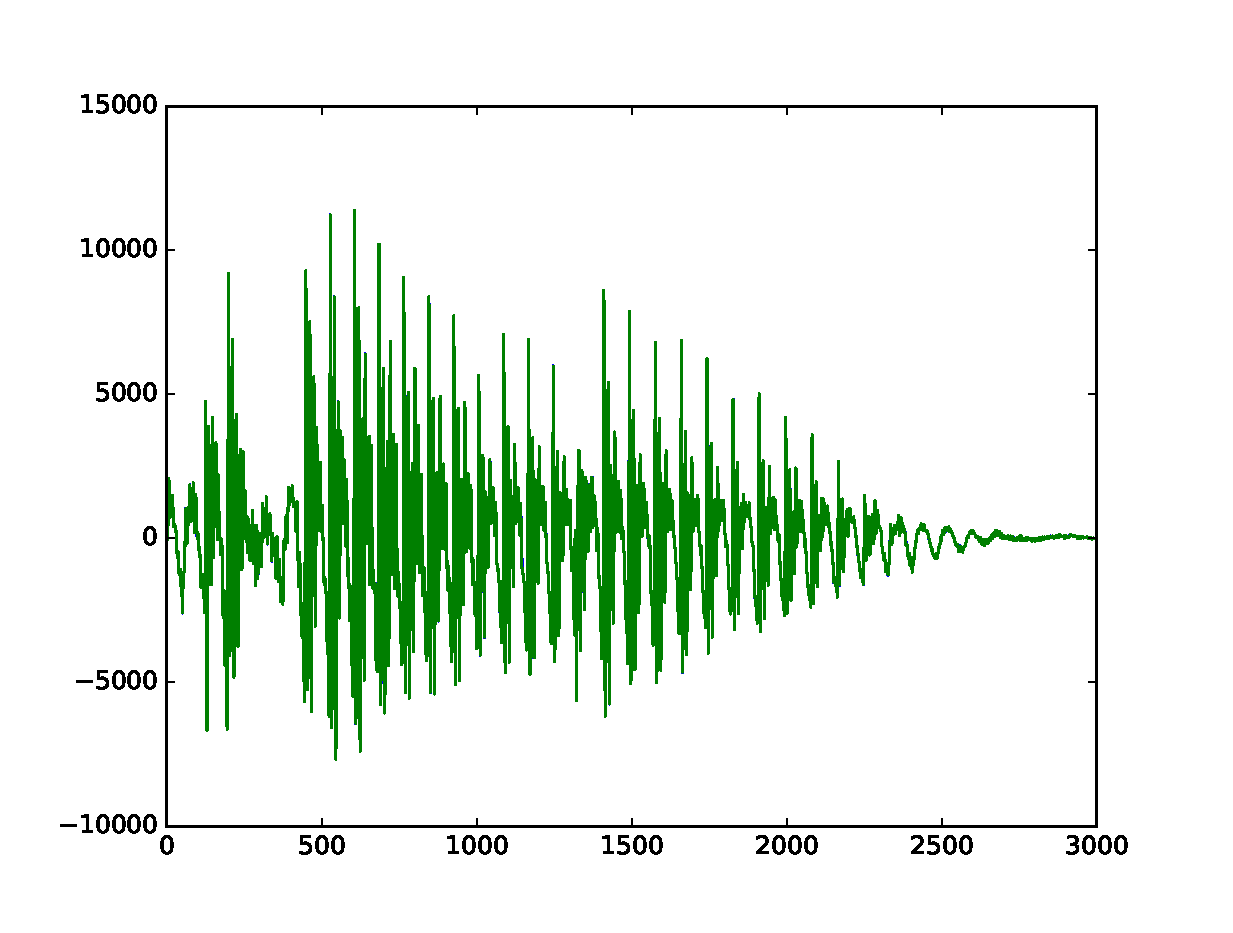
\includegraphics[width=0.8\textwidth]{a1.eps}
\end{frame}

\begin{frame}
  \frametitle{\insertsection}
  \framesubtitle{Выборка сигнала соответствующего звуку ``a'' номер 2}
  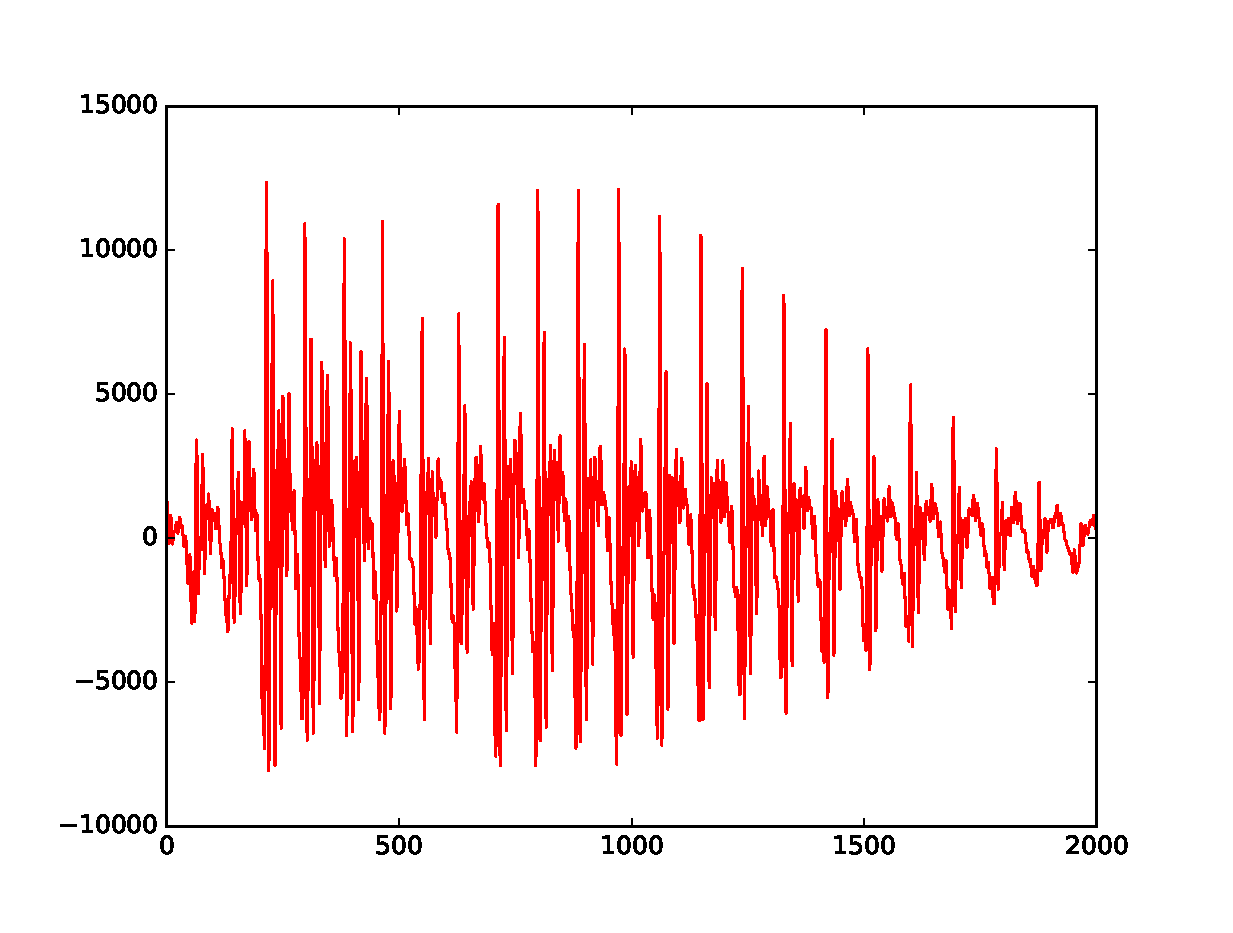
\includegraphics[width=0.8\textwidth]{a2.eps}
\end{frame}

\begin{frame}
  \frametitle{\insertsection}
  \framesubtitle{Совмещение сигналов двух выборок}
  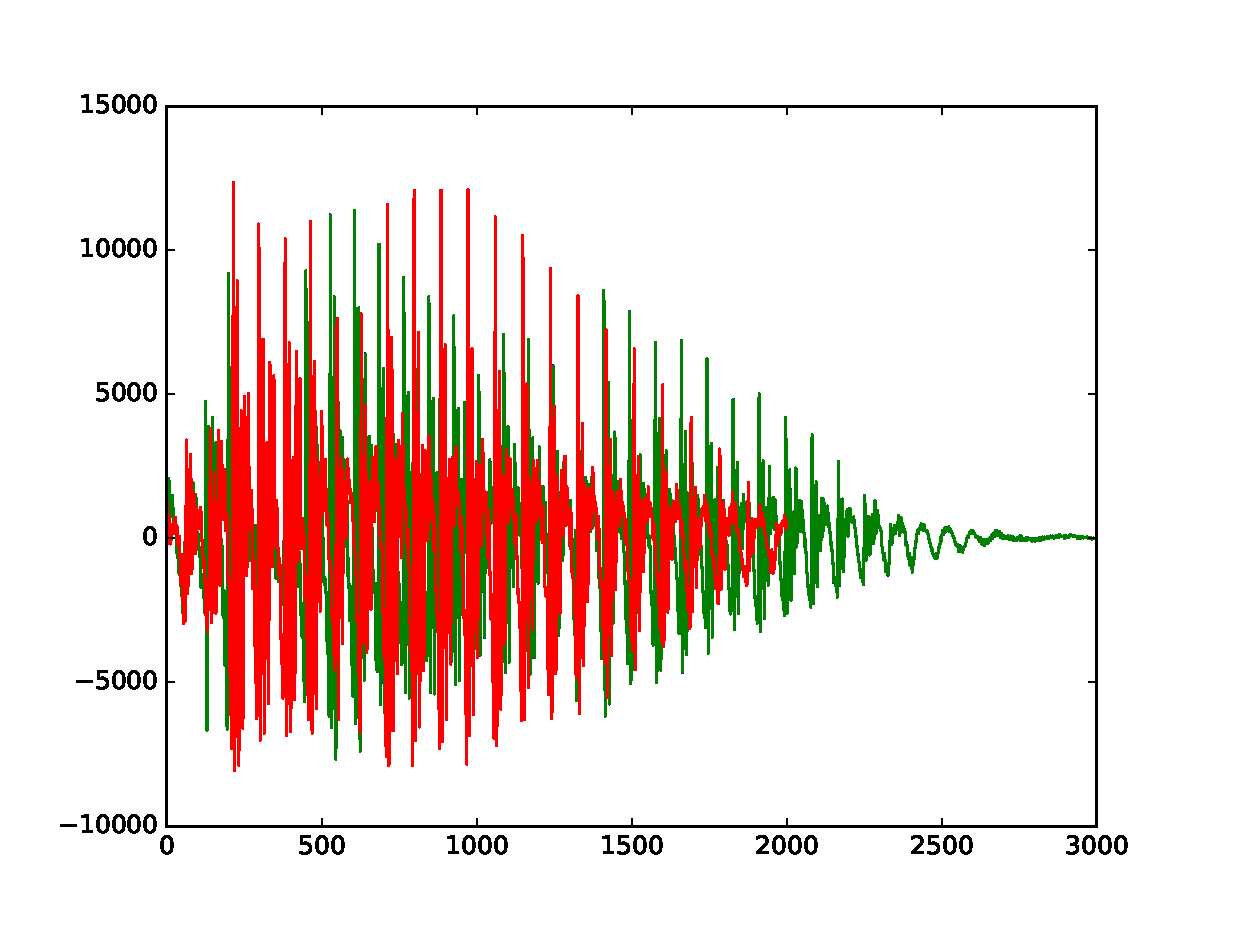
\includegraphics[width=0.8\textwidth]{a1a2.eps}
\end{frame}

\begin{frame}
  \frametitle{\insertsection}
  \framesubtitle{\insertsubsection}
  
  \begin{center}
  Теория вероятности как аппарат для описания закономерность в случайных событиях. 
  \end{center} \pause
  \begin{itemize}
  \item Случайный вектор: $ \mathbf{X} = [\mathbf{x}_0\, \mathbf{x}_1 \ldots \mathbf{x}_{N - 1}]^T $
  \end{itemize}

\end{frame}

\section{Случайные векторы}
\subsection{Функция вероятности и функция плотности вероятности}

\begin{frame}
  \frametitle{\insertsection}
  \framesubtitle{\insertsubsection}
  \begin{equation*}
   P(x_1, \ldots, x_n) = Pr\{\mathbf{x}_1 \le x_1, \ldots \mathbf{x}_n \le x_n \} 
  \end{equation*}
  
  \begin{align*}
    p(X) &=
    \lim_{\Delta X \rightarrow 0}
    \frac{
      Pr\{x_1 \textless \mathbf{x}_1 \le x_1 + \Delta x_1, \ldots x_n \textless \mathbf{x}_n \le x_n + \Delta x_n \}
    }
         {\Delta x_1 \, \ldots \, \Delta x_n} \\
         &= \partial^n P(X) / \partial x_1 \, \ldots \, \partial x_n
  \end{align*}
  
  \begin{equation*}
   P(X) = \int_{-\infty}^{X} p(Y) dY = \int_{-\infty}^{x_1} \, \ldots \int_{-\infty}^{x_n} p(y_1, \ldots, y_n) d y_1 \, \ldots \, y_n
  \end{equation*}


\end{frame}

\subsection{Параметры распределения (моменты): математическое ожидание}

\begin{frame}
  \frametitle{\insertsection}
  \framesubtitle{\insertsubsection}
  
  \begin{equation*}
    M = E\{ \mathbf{X} \} = \int X p(X) dX
  \end{equation*}
  $i$ - ая компонента вектора математического ожидания:
  \begin{equation*}
    m_i = \int_{-\infty}^{\infty} x_i p(x_i) dx_i
  \end{equation*}

  \begin{equation*}
    p(x_i) = \underbrace{\int_{-\infty}^{\infty} \ldots \int_{-\infty}^{\infty}}_{n - 1} p(X) dx_1 \ldots d x_{i - 1} d x_{i + 1} \ldots d x_n
  \end{equation*}

\end{frame}

\subsection{Параметры рапределения (моменты): матрица ковариации}

\begin{frame}
  \frametitle{\insertsection}
  \framesubtitle{\insertsubsection}
  \begin{multline*}
    \Sigma = E\{(\mathbf{X} - M)(\mathbf{X} - M)^T\} =\\
    E \left\{
    \begin{bmatrix}
      \mathbf{x_1} - m_1\\
      \vdots\\
      \mathbf{x_n} - m_n
    \end{bmatrix}
    \begin{bmatrix}
      \mathbf{x_1} - m_1 & \ldots & \mathbf{x_n} - m_n
    \end{bmatrix}
    \right\} =\\
      E \left\{
      \begin{bmatrix}
        (\mathbf{x_1} - m_1)(\mathbf{x_1} - m_1) & \ldots & (\mathbf{x_1} - m_1)(\mathbf{x_n} - m_n)\\
        \vdots & &\\
        (\mathbf{x_n} - m_n)(\mathbf{x_1} - m_1) & \ldots & (\mathbf{x_n} - m_n)(\mathbf{x_n} - m_n) 
      \end{bmatrix}
      \right\} =\\
      \begin{bmatrix}
        E\{(\mathbf{x_1} - m_1)(\mathbf{x_1} - m_1)\} & \ldots & E\{(\mathbf{x_1} - m_1)(\mathbf{x_n} - m_n)\}\\
        \vdots & &\\
        E\{(\mathbf{x_n} - m_n)(\mathbf{x_1} - m_1)\} & \ldots & E\{(\mathbf{x_n} - m_n)(\mathbf{x_n} - m_n)\} 
      \end{bmatrix}
  \end{multline*}

\end{frame}

\section{Многомерное гауссово (нормальное) распределение}

\begin{frame}
  \frametitle{\insertsection}
  \framesubtitle{\insertsubsection}
  
  \begin{equation*}
    N_X(M, \Sigma) = \frac{1}{(2 \pi )^{n/2} | \Sigma |^{1/2} }
    \exp(-\frac{1}{2} d^2(X))
  \end{equation*}
  где $M$ --- это вектор математического ожидания, $\Sigma$ --- матрица ковариации, \pause
  \begin{align*}
    d^2(X) &= (X - M)^T \Sigma^{-1} (X - M)\\
           &= tr\{\Sigma^{-1} (X - M)(X - M)^T\}\\
           &=\sum_{i = 1}^{n}\sum_{j = 1}^{n} h_{ij}(x_i - m_i)(x_j - m_j)
  \end{align*}

  \begin{itemize}
    \item $tr\{M\}$ --- след матрицы
    \item $h_{ij}$ --- диагональный элемент матрицы $\Sigma$
  \end{itemize}


\end{frame}

\subsection{Свойства}

\begin{frame}
  \frametitle{\insertsection}
  \framesubtitle{\insertsubsection}

  \begin{enumerate}
    \item Полностью определяется вектором математического ожидания и матрицей ковариации \pause
    \item Если элементы случайного вектора не коррелированы, то они и независимы \pause
    \item Распределение по отдельным элементам также является нормальным \pause
    \item Остается нормальным после линейного невырожденного преобразования \pause
    \item Центральная предельная теорема
  \end{enumerate}

\end{frame}

\subsection{Графическое представление}

\begin{frame}
  \frametitle{\insertsection}
  \framesubtitle{\insertsubsection}
  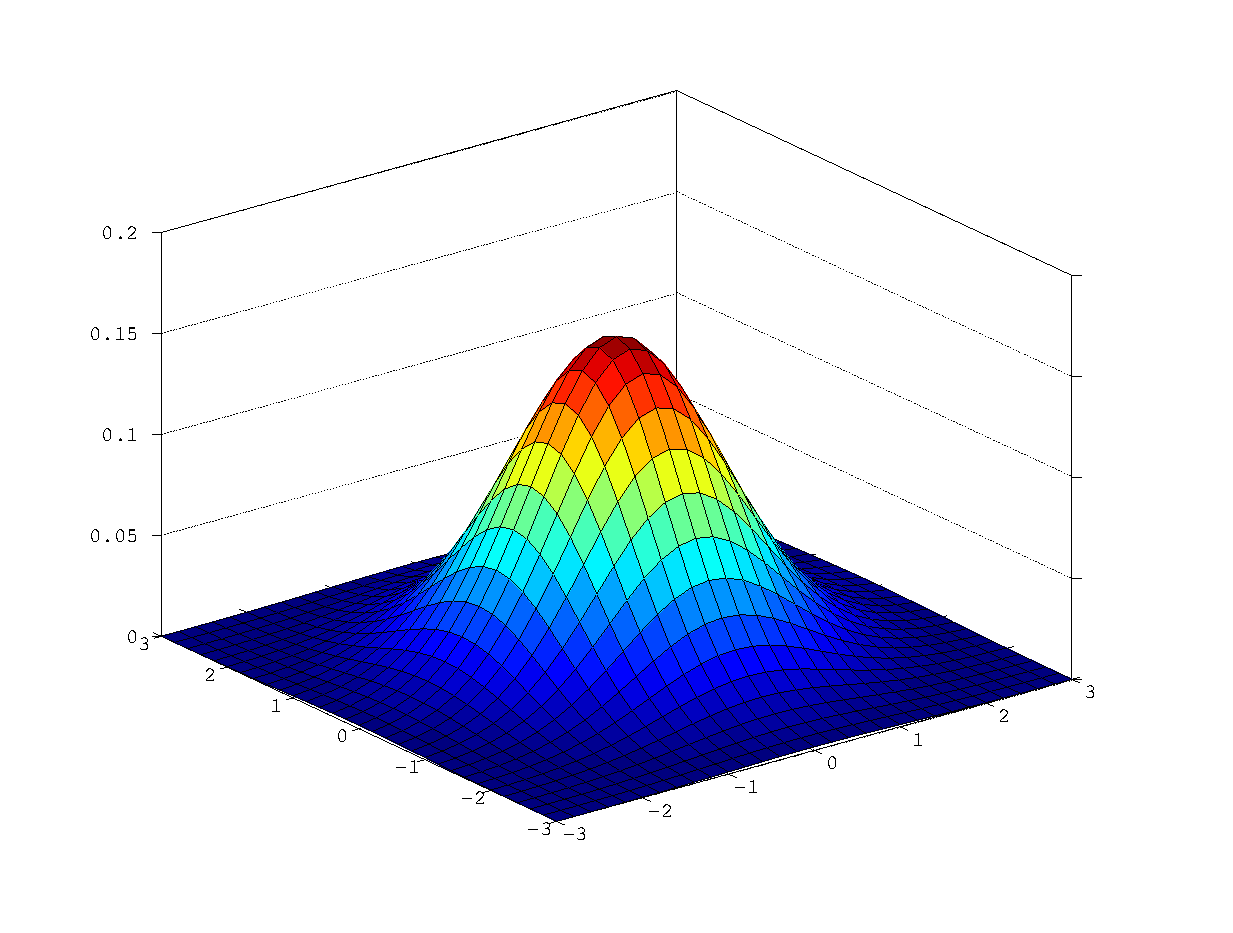
\includegraphics[width=0.8\textwidth]{normal.eps}  
\end{frame}

\section{Байесовский классификатор}
\subsection{Проверка гипотез для двух классов}

\begin{frame}
  \frametitle{\insertsection}
  \framesubtitle{\insertsubsection}
  %% Для понимания рассматриваем самый простой вариант проблемы
  
  \begin{itemize}
    \item есть два класса: $\omega_1$ и $\omega_2$ \pause
    \item распределение плотности вероятности известно для каждого из них \pause
    \item дан произвольный вектор $X$
  \end{itemize}
  Необходимо определить к какому из двух классов относится вектор $X$!
  
\end{frame}

\begin{frame}
  \frametitle{\insertsection}
  \framesubtitle{\insertsubsection}
  Суть метода проста:
  \begin{equation*}
    \omega =
    \begin{cases}
      \omega_1 & \text{if } P(w_1 | X) \textgreater P(w_2 | X),\\
      \omega_2 & \text{if } P(w_1 | X) \textless P(w_2 | X),
    \end{cases}
  \end{equation*}
\end{frame}

\subsection{Апостериорная вероятность}

\begin{frame}
  \frametitle{\insertsection}
  \framesubtitle{\insertsubsection}
  
  \begin{itemize}
  \item $\displaystyle P(\omega_i | X) = \frac{P(X | \omega_i) P(\omega_i)}{P(X)} $ \pause
  \item $\displaystyle
    \omega =
    \begin{cases}
      \omega_1 & \text{if } P(X | \omega_1) P(\omega_1) \textgreater P(X | \omega_2) P(\omega_2),\\
      \omega_2 & \text{if } P(X | \omega_1) P(\omega_1) \textless P(X | \omega_2) P(\omega_2)
    \end{cases}$ \pause
  \item $\displaystyle \ell(X) = \frac{P(X | \omega_1)}{P(X | \omega_2)} $
    \pause
  \item $\displaystyle
    \omega =
    \begin{cases}
      \omega_1 & \text{if } \ell(X) \textgreater P(\omega_2) / P(\omega_1),\\
      \omega_2 & \text{if } \ell(X) \textless P(\omega_2) / P(\omega_1)
    \end{cases}$ \pause
  \item $\displaystyle h(x) = -\ln \ell(X) = -\ln p(X | \omega_1) + \ln p(X | \omega_2) $
  \end{itemize}
\end{frame}

%% \subsection{Ограничение сверху на Байесовскую ошибку}
\subsection{Пример. Нормальное распределение}

\begin{frame}
  \frametitle{\insertsection}
  \framesubtitle{\insertsubsection}
  
  \begin{multline*}
    h(X) = -\ln \ell(X) =\\
    \frac12 (X - M_1)^T \Sigma_1^{-1}(X - M_1)\\
    - \frac12 (X - M_2)^T \Sigma_2^{-1}(X - M_2) + \frac12 \ln \frac{\Sigma_1}{\Sigma_2}
  \end{multline*}

\end{frame}

\begin{frame}
  \frametitle{\insertsection}
  \framesubtitle{\insertsubsection}
  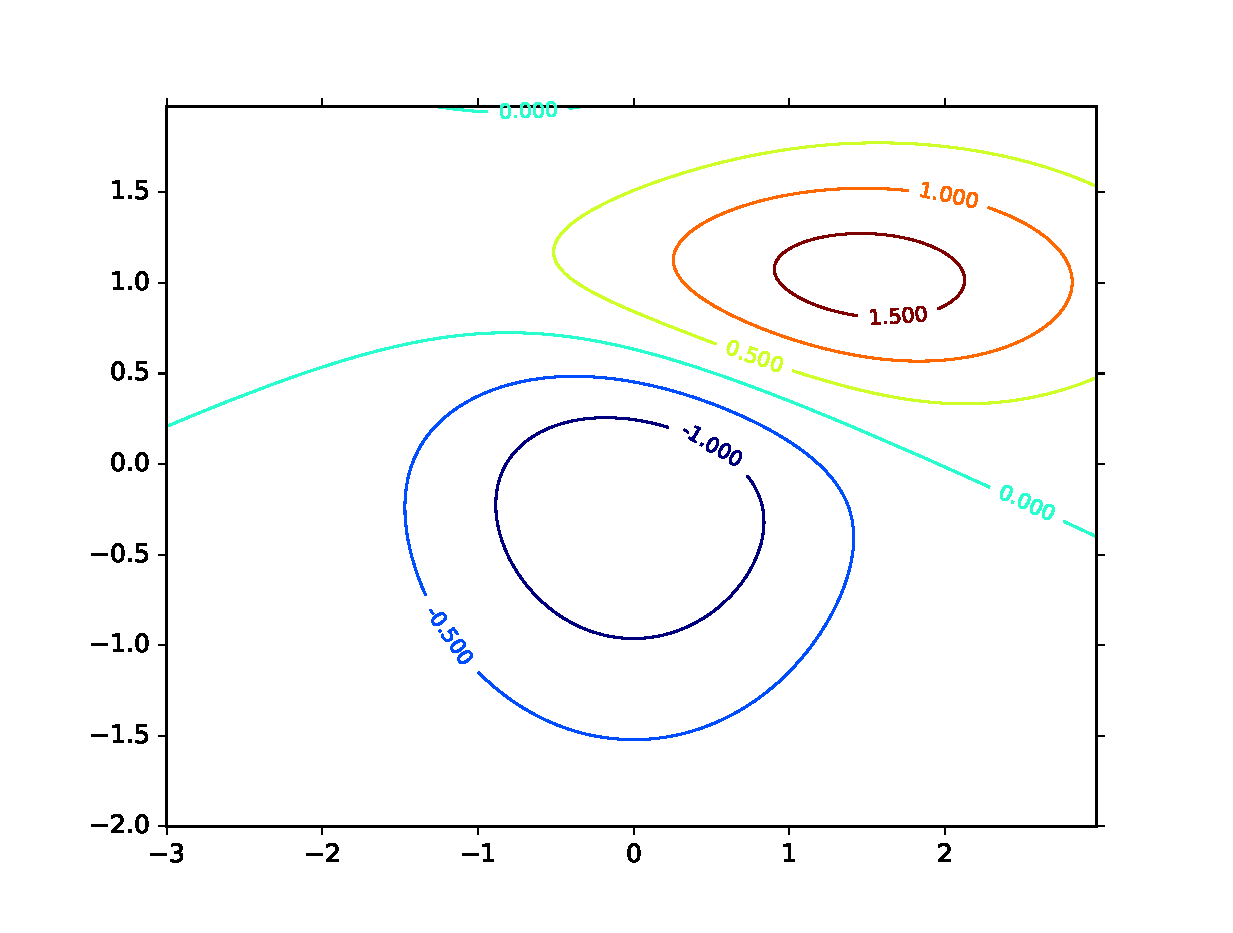
\includegraphics[width=0.8\textwidth]{border.eps}  
\end{frame}

\end{document}
